\documentclass{infufrgs}
\usepackage[utf8]{inputenc}
\usepackage{framed}
\usepackage{amsmath}
\usepackage{graphicx} 
\usepackage{listings}
\usepackage{fancyvrb}
\usepackage{booktabs}
\usepackage{xcolor}
\usepackage{float}

% Configuração para snippets de código
\lstset{
    language=C++,
    basicstyle=\ttfamily\scriptsize,
    keywordstyle=\color{blue},
    stringstyle=\color{red},
    commentstyle=\color{green!50!black},
    numbers=left,
    numberstyle=\tiny\color{gray},
    stepnumber=1,
    numbersep=5pt,
    backgroundcolor=\color{gray!5},
    showspaces=false,
    showstringspaces=false,
    frame=single,
    rulecolor=\color{black!30},
    breaklines=true,
    breakatwhitespace=true,
    tabsize=2
}

\colorlet{shadecolor}{orange!15}

\title{Relatório de Análise Experimental: Algoritmos de Fluxo Máximo}
\author{Rodrigues}{Juliana} 

\begin{document}

\maketitle

\chapter{Relatório do Experimento}

%==================================================
% INTRODUÇÃO
%==================================================
\section{Introdução}
Este relatório descreve a avaliação empírica de seis algoritmos de fluxo máximo $s-t$ da família Ford-Fulkerson[cite: 1, 3]. O objetivo é verificar a complexidade experimental, comparando o desempenho real com os limites teóricos pessimistas. 

A análise foca na "inadequação" (defeito) das métricas teóricas:
\begin{itemize}
    \item \textbf{Inadequação de Fases ($r$):} Razão entre fases reais e o limite teórico ($F/\overline{F}$). 
    \item \textbf{Defeito de Vértices ($\overline{s}$):} Fração média de vértices tocados por fase. 
    \item \textbf{Defeito de Arcos ($\overline{t}$):} Fração média de arcos avaliados por fase. 
\end{itemize}


%==================================================
% INSTÂNCIAS DE TESTE
%==================================================
\section{Instâncias de Teste e Plano de Experimentos}

Os experimentos foram conduzidos com o gerador de grafos \texttt{washington} (versão \texttt{new\_washington.c}), que produz redes de fluxo no formato DIMACS. A semente do gerador é fixa em $1$ (\texttt{InitRandom(1)}), tornando todos os experimentos \textbf{determinísticos e reprodutíveis}.

\subsection{Estrutura Geral dos Grafos Gerados}

Para os tipos 6–8, o gerador recebe os parâmetros \texttt{dim1} ($n$), \texttt{dim2} ($m$), \texttt{deg} e \texttt{range}, e constrói uma rede em grade com $n \times m + 2$ vértices no total (incluindo fonte $s$ e sorvedouro $t$). Cada vértice interno possui exatamente \texttt{deg} arestas de saída, sorteadas aleatoriamente dentre os vizinhos à frente. As arestas incidentes à fonte e ao sorvedouro têm capacidade $\texttt{deg} \times \texttt{range}$, garantindo que o gargalo da rede esteja nos arcos internos.

\subsection{Famílias de Grafos}

Foram avaliadas duas famílias topológicas, ambas geradas com \texttt{dim1 = 2}:

\textbf{BasicLine (Tipo 6):} Gerada por \texttt{BasicLine(n, m, deg, range)}. Os deslocamentos de aresta são amostrados uniformemente em $[1,\, m \cdot \texttt{deg}]$, e as capacidades são sorteadas uniformemente em $[1, \texttt{range}]$. Representa redes com estrutura regular e capacidades homogêneas.

\textbf{DoubleExpLine (Tipo 8):} Gerada por \texttt{DExponentialLine(n, m, deg, range)}. Os deslocamentos são amostrados em $[-m \cdot \texttt{deg},\, m \cdot \texttt{deg}]$ (permitindo arcos que ``saltam'' para trás e para frente), e as capacidades seguem um esquema de \textbf{decaimento exponencial}: arcos com deslocamento curto recebem capacidades altas (até $10^6$), enquanto arcos com deslocamento longo recebem capacidades baixas (mínimo $2$), conforme o vetor \texttt{Range[]}. Isso produz redes com estrutura mais complexa e heterogeneidade de capacidades, representando instâncias estruturalmente mais desafiadoras.

\subsection{Experimento A: Impacto da Densidade (\texorpdfstring{$n$}{n} fixo, \texorpdfstring{$m$}{m} crescente)}

O tamanho da rede é mantido fixo com \texttt{dim1 = 2} e \texttt{dim2 = 2500}, produzindo $n = 2 \times 2500 + 2 = 5002$ vértices. O grau médio de saída varia no conjunto $\{2, 5, 10, 20, 40\}$, aumentando progressivamente o número de arcos $m$. O objetivo é isolar o efeito da densidade sobre o número de fases, operações e tempo de execução, mantendo a escala da rede constante.

\subsection{Experimento B: Impacto da Escala (Densidade fixa, \texorpdfstring{$n$}{n} crescente)}

O grau médio de saída é fixado em $\texttt{deg} = 10$, enquanto \texttt{dim2} varia no conjunto $\{500, 1000, 2500, 5000, 10000\}$, produzindo redes com $n \in \{1002, 2002, 5002, 10002, 20002\}$ vértices. O objetivo é verificar o crescimento assintótico real dos algoritmos em função da escala da rede.

\subsection{Métricas Coletadas e Limites Teóricos}

Para cada par (algoritmo, instância), o experimento registra: número de fases $F$, número total de vértices tocados, número total de arcos avaliados, e tempo de execução em milissegundos. A partir dessas medidas, calculam-se as seguintes métricas de defeito:

\begin{equation}
    r = \frac{F}{\overline{F}}, \qquad
    \overline{s} = \frac{\text{vértices tocados}}{n \cdot D}, \qquad
    \overline{t} = \frac{\text{arcos avaliados}}{m \cdot F}
\end{equation}

\noindent onde $D$ é o divisor por fase — igual a $F$ para todos os algoritmos, exceto para Dinitz, onde $D$ corresponde ao número total de iterações internas do fluxo bloqueante, refletindo que cada DFS toca um subconjunto de vértices independente.

O valor de $C$ (fluxo máximo) é obtido na primeira execução (Edmonds-Karp) e reutilizado como referência para os limites dos demais algoritmos. Os limites teóricos $\overline{F}$ são:

\begin{table}[H]
\centering
\caption{Limites teóricos de fases $\overline{F}$ por algoritmo.}
\begin{tabular}{llll}
\toprule
\textbf{Algoritmo} & \textbf{Sigla} & \textbf{Complexidade} & \textbf{$\overline{F}$} \\
\midrule
Edmonds-Karp                & EK   & $O(nm^2)$           & $nm/2$        \\
Ford-Fulkerson DFS          & FF   & $O(mC)$             & $C$           \\
Ford-Fulkerson RDFS         & RDFS & $O(mC)$             & $C$           \\
Fattest Path                & FP   & $O(m^2 \log C)$     & $m \log_2 C$  \\
Escalonamento de Capacidade & EC   & $O(m^2 \log C)$     & $m \log_2 C$  \\
Dinitz                      & Di   & $O(n^2 m)$          & $n$           \\
\bottomrule
\end{tabular}
\end{table}

%==================================================
% IMPLEMENTAÇÃO
%==================================================
\section{Algoritmos e Análise de Complexidade}
Abaixo, detalhamos as implementações e as regiões críticas do código que definem sua complexidade.

\subsection{1. Ford-Fulkerson (DFS)}
Usa Busca em Profundidade (DFS) com complexidade $O(m \cdot C)$. No pior caso, cada fase aumenta o fluxo em apenas 1 unidade.
\begin{lstlisting}[caption={Busca de caminho via DFS em FordFulkersonDFS.cpp}]
    for (size_t i = 0; i < network.adj_list[u].size(); ++i) {
        e_touched++; 
        Edge& edge = network.adj_list[u][i];
        long long residual = network.get_residual_capacity(edge);
        if (!visited[edge.to] && residual > 0) {
            long long bottleneck = dfs(network, edge.to, t, std::min(current_flow, residual), visited, v_touched, e_touched);
\end{lstlisting}

\subsection{2. Randomized Ford-Fulkerson (RDFS)}
Mantém a complexidade $O(m \cdot C)$, mas utiliza embaralhamento para evitar casos patológicos determinísticos.
\begin{lstlisting}[caption={Embaralhamento de arestas em FordFulkersonRandDFS.cpp}]
    std::shuffle(indices.begin(), indices.end(), g); 
    for (size_t idx = 0; idx < network.adj_list[u].size(); ++idx) {
        size_t i = indices[idx]; 
\end{lstlisting}

\subsection{3. Edmonds-Karp (BFS)}
Garante tempo fortemente polinomial $O(nm^2)$ ao usar Busca em Largura (BFS) para encontrar o caminho mais curto.
\begin{lstlisting}[caption={Travessia BFS em EdmondsKarp.cpp}]
    while (!q.empty() && !reached_sink) {
        int u = q.front(); q.pop();
        for (size_t i = 0; i < network.adj_list[u].size(); ++i) {
            if (parent_node[edge.to] == -1 && network.get_residual_capacity(edge) > 0) {
                parent_node[edge.to] = u;
\end{lstlisting}

\subsection{4. Algoritmo de Dinitz (Di)}
Alcança $O(n^2m)$ usando grafos de níveis e fluxos bloqueantes. O uso do array \texttt{ptr} evita revisitar caminhos saturados na mesma fase.
\begin{lstlisting}[caption={Poda de busca no grafo de níveis em Dinitz.cpp}]
    for (int& cid = ptr[u]; cid < network.adj_list[u].size(); ++cid) {
        Edge& edge = network.adj_list[u][cid];
        if (level[u] + 1 != level[edge.to] || res == 0) continue;
\end{lstlisting}

\subsection{5. Escalonamento de Capacidade (EC)}
Possui complexidade $O(m^2 \log C)$, limitando a busca a arestas com capacidade residual superior a um valor $\Delta$.
\begin{lstlisting}[caption={Controle de Delta em CapacityScaling.cpp}]
    while (delta >= 1) {
        while (path_found) {
             if (parent_node[edge.to] == -1 && network.get_residual_capacity(edge) >= delta) {
\end{lstlisting}

\subsection{6. Caminho Mais Gordo (FP)}
Usa uma variação de Dijkstra para maximizar o gargalo do caminho, com custo de fase $O(m \log n)$ devido ao uso de Heap.
\begin{lstlisting}[caption={Uso de Priority Queue em FattestPath.cpp}]
    while (!pq.is_empty()) {
        int u = pq.extract_max();
        if (bottleneck > max_cap[edge.to]) {
            pq.update_key(edge.to, bottleneck); 
\end{lstlisting}



%==================================================
% RESULTADOS
%==================================================
\section{Resultados Experimentais e Análise Gráfica}

\subsection{Família de Grafos: DoubleExpLine}

\subsubsection{Experimento A: Impacto de Densidade (n fixo, m crescente)}

\begin{figure}[H]
    \centering
    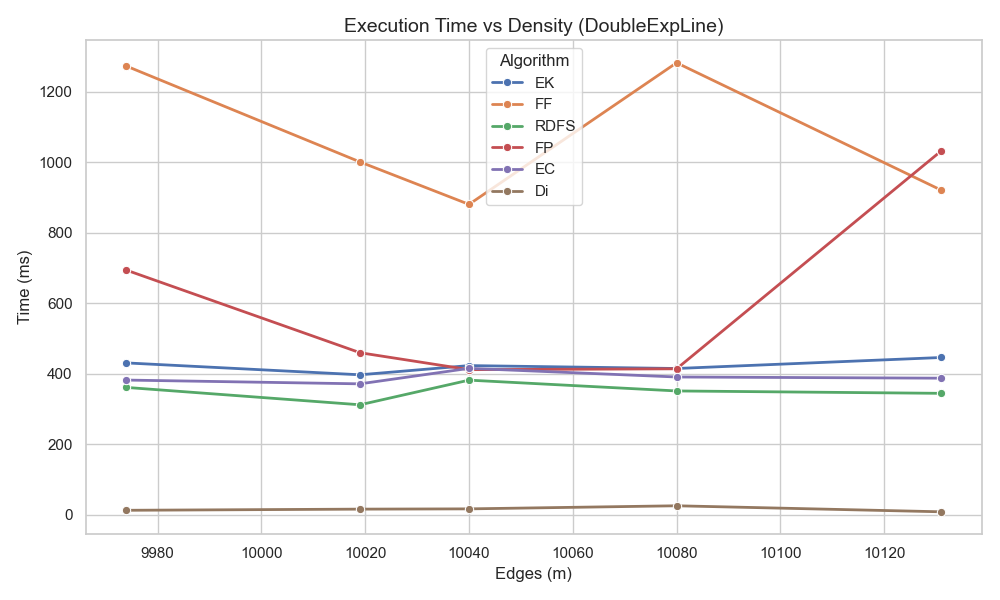
\includegraphics[width=0.75\textwidth]{Images/time_density_DoubleExpLine.png}
    \caption{Tempo de Execução vs Densidade (DoubleExpLine): Mostra que Dinitz forma a curva mais baixa e estável, enquanto o Fattest Path cresce mais rápido devido ao custo do Heap. }
\end{figure}

\begin{figure}[H]
    \centering
    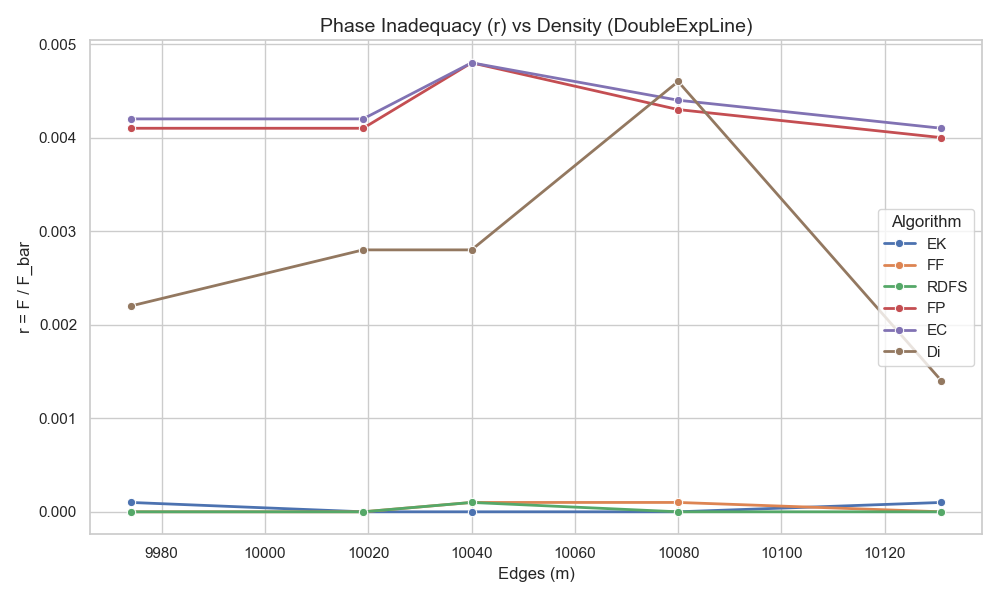
\includegraphics[width=0.75\textwidth]{Images/r_density_DoubleExpLine.png}
    \caption{Razão de Fases ($r$) vs Densidade (DoubleExpLine): Demonstra que as fases reais executadas são uma fração mínima do limite teórico pessimista, tendendo a zero com o aumento de $m$. }
\end{figure}

\begin{figure}[H]
    \centering
    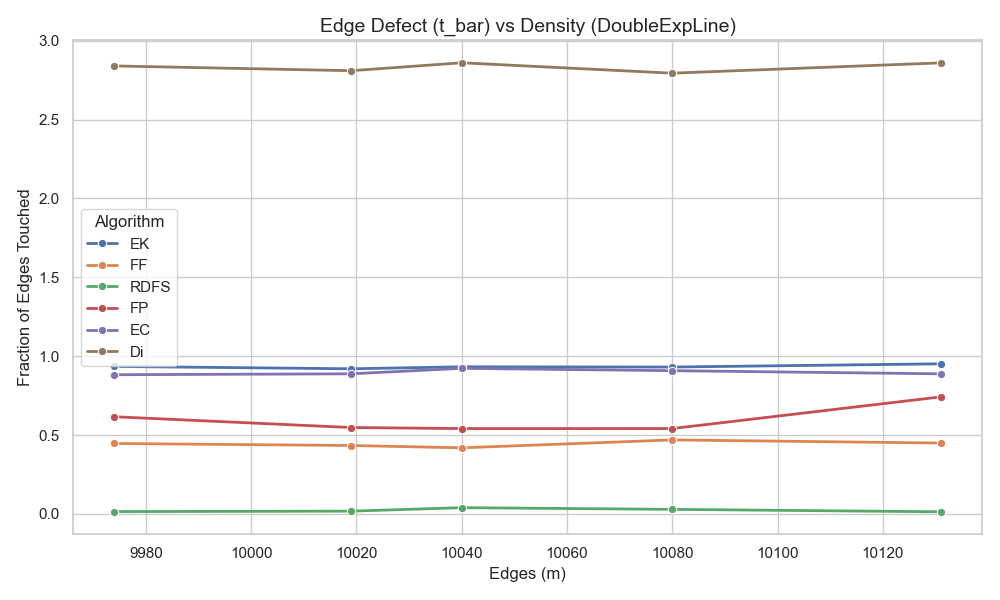
\includegraphics[width=0.75\textwidth]{Images/t_bar_density_DoubleExpLine.png}
    \caption{Defeito de Arcos ($\overline{t}$) vs Densidade (DoubleExpLine): Revela a "personalidade" das buscas; EK (BFS) toca quase todos os arcos ($\approx 1.0$), enquanto FF (DFS) toca muito menos. }
\end{figure}

\subsubsection{Experimento B: Impacto de Escala (Densidade fixa, n crescente)}

\begin{figure}[H]
    \centering
    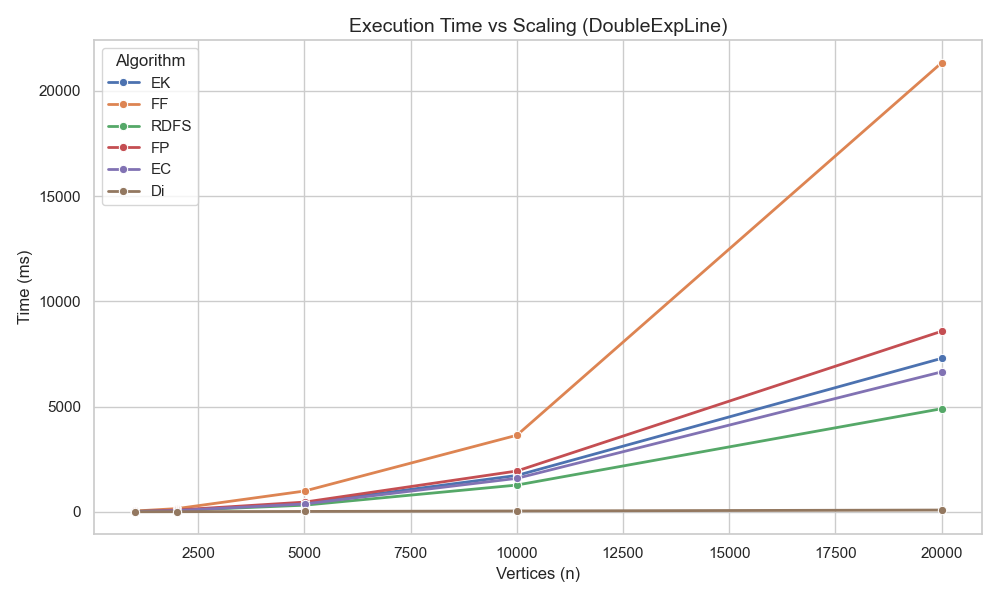
\includegraphics[width=0.75\textwidth]{Images/time_scaling_DoubleExpLine.png}
    \caption{Tempo de Execução vs Escala (DoubleExpLine): Dinitz confirma sua superioridade em escala, mantendo a curva de crescimento mais suave. }
\end{figure}

\begin{figure}[H]
    \centering
    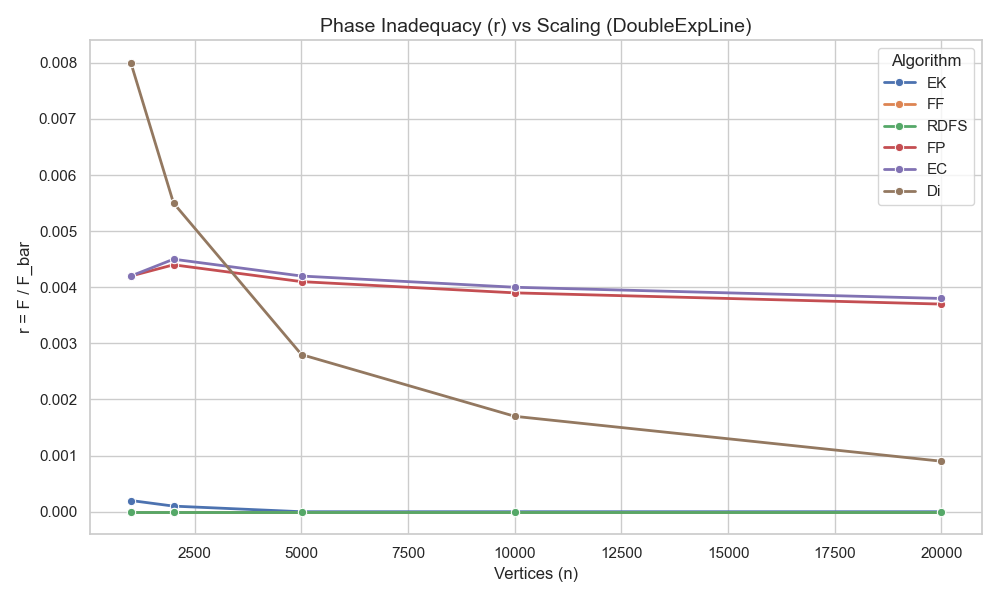
\includegraphics[width=0.75\textwidth]{Images/r_scaling_DoubleExpLine.png}
    \caption{Razão de Fases ($r$) vs Escala (DoubleExpLine): Prova visual de que o limite teórico explode enquanto o número real de fases cresce muito lentamente. }
\end{figure}

\begin{figure}[H]
    \centering
    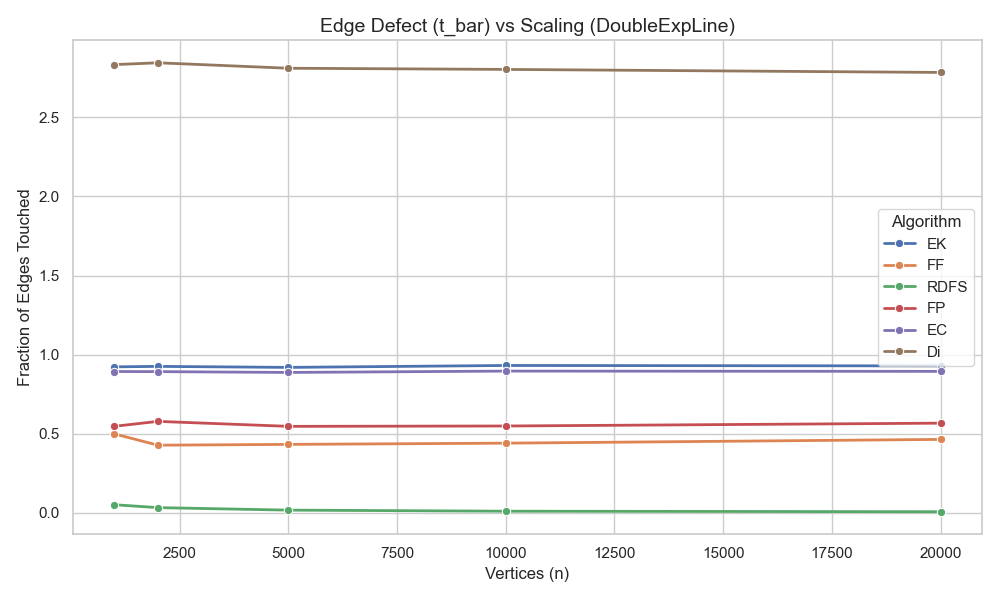
\includegraphics[width=0.75\textwidth]{Images/t_bar_scaling_DoubleExpLine.png}
    \caption{Defeito de Arcos ($\overline{t}$) vs Escala (DoubleExpLine): Dinitz apresenta $\overline{t} > 1$ pois toca mais arestas para construir o grafo de níveis e fluxos bloqueantes. }
\end{figure}

\subsection{Família de Grafos: BasicLine}

\subsubsection{Experimento A: Impacto de Densidade (n fixo, m crescente)}

\begin{figure}[H]
    \centering
    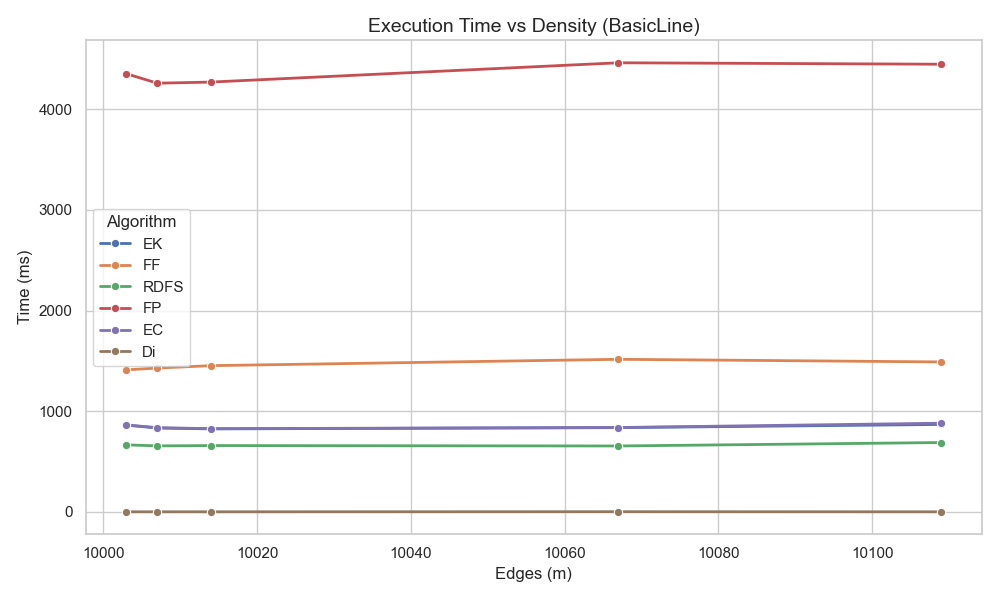
\includegraphics[width=0.75\textwidth]{Images/time_density_BasicLine.png}
    \caption{Tempo de Execução vs Densidade (BasicLine): Reflete a sobrecarga residual de estruturas de dados (como Filas de Prioridade no FP) mesmo em grafos mais simples. }
\end{figure}

\begin{figure}[H]
    \centering
    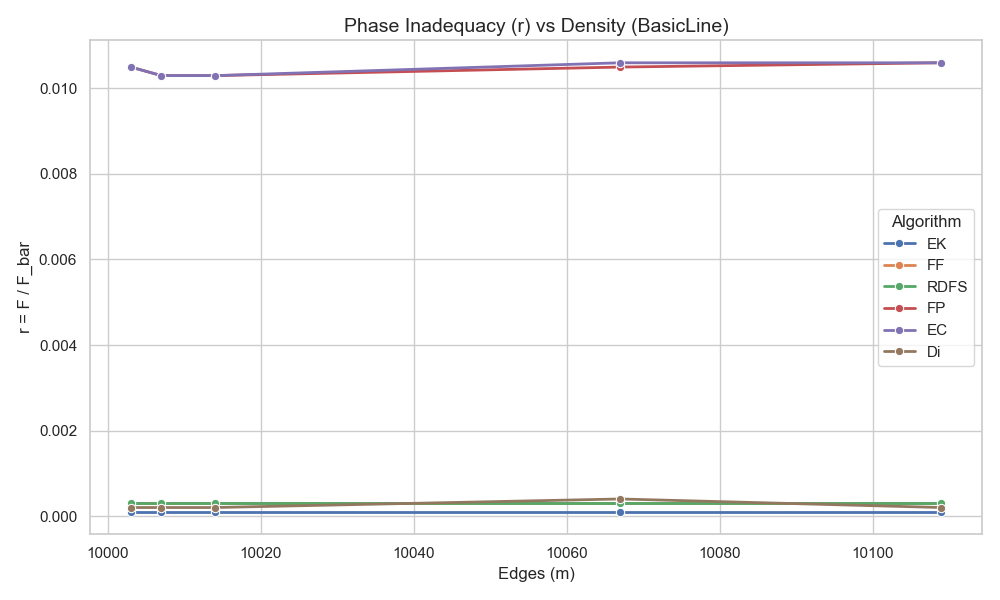
\includegraphics[width=0.75\textwidth]{Images/r_density_BasicLine.png}
    \caption{Razão de Fases ($r$) vs Densidade (BasicLine): Confirma a inadequação dos limites teóricos independentemente da topologia do grafo. }
\end{figure}

\begin{figure}[H]
    \centering
    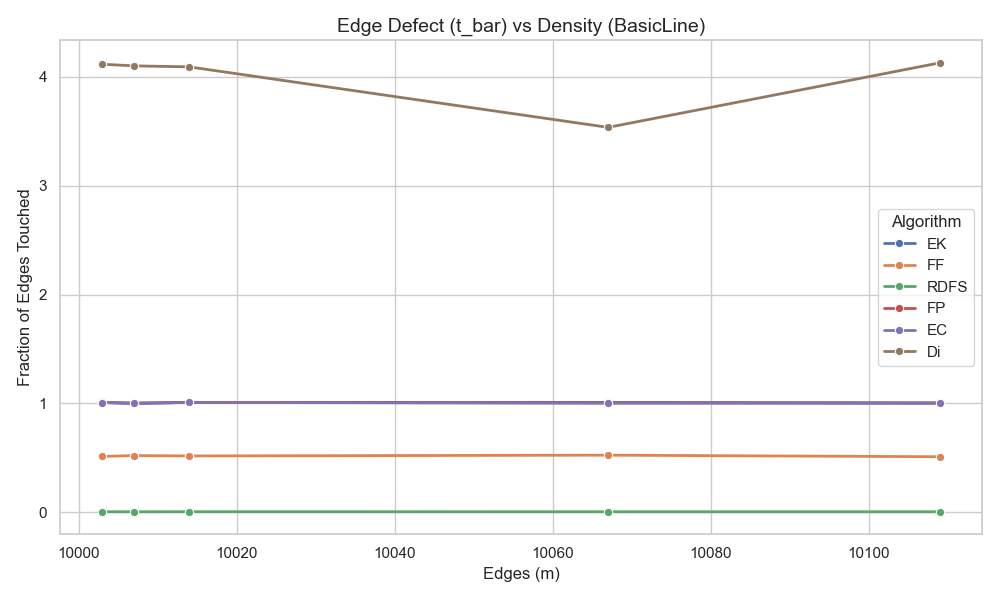
\includegraphics[width=0.75\textwidth]{Images/t_bar_density_BasicLine.png}
    \caption{Defeito de Arcos ($\overline{t}$) vs Densidade (BasicLine): Mantém a consistência comportamental dos algoritmos; EK explorando amplamente e FF/RDFS explorando pontualmente. }
\end{figure}

\subsubsection{Experimento B: Impacto de Escala (Densidade fixa, n crescente)}

\begin{figure}[H]
    \centering
    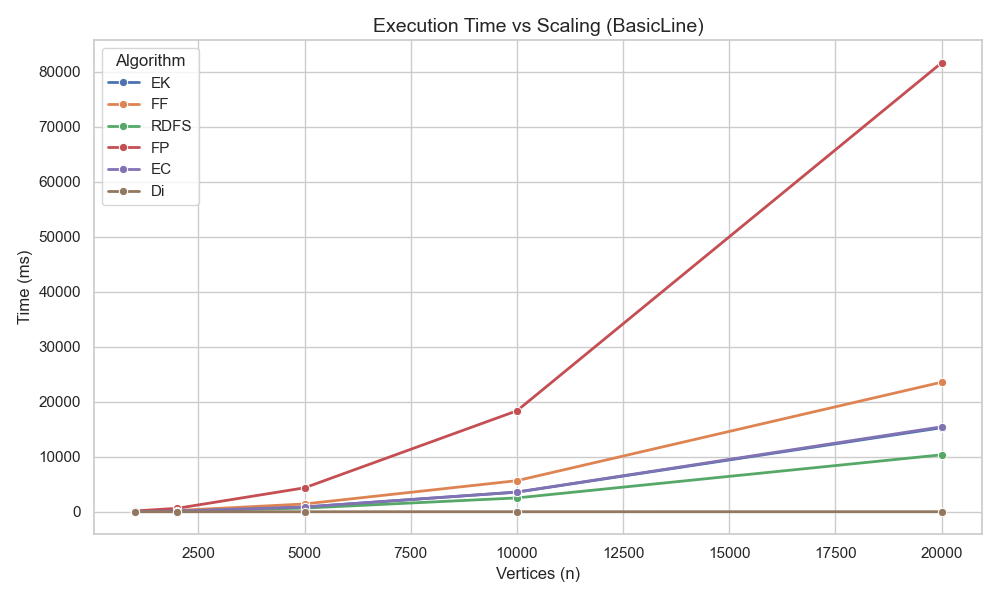
\includegraphics[width=0.75\textwidth]{Images/time_scaling_BasicLine.png}
    \caption{Tempo de Execução vs Escala (BasicLine): Visualiza o crescimento assintótico real, onde Dinitz e Edmonds-Karp apresentam ótimo desempenho. }
\end{figure}

\begin{figure}[H]
    \centering
    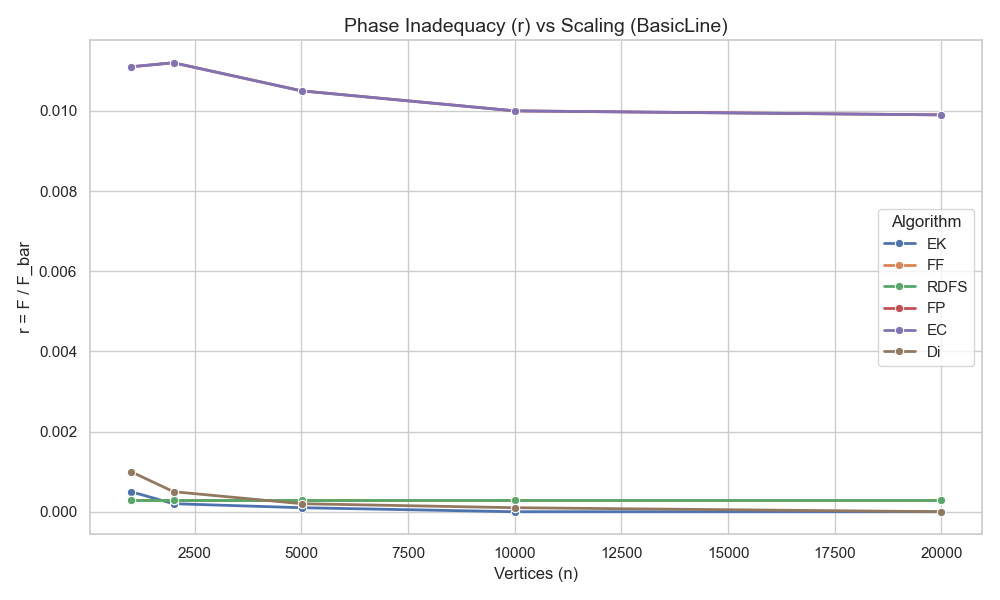
\includegraphics[width=0.75\textwidth]{Images/r_scaling_BasicLine.png}
    \caption{Razão de Fases ($r$) vs Escala (BasicLine): Reforça que o "defeito" das fórmulas de complexidade pessimista aumenta proporcionalmente ao tamanho da rede. }
\end{figure}

\begin{figure}[H]
    \centering
    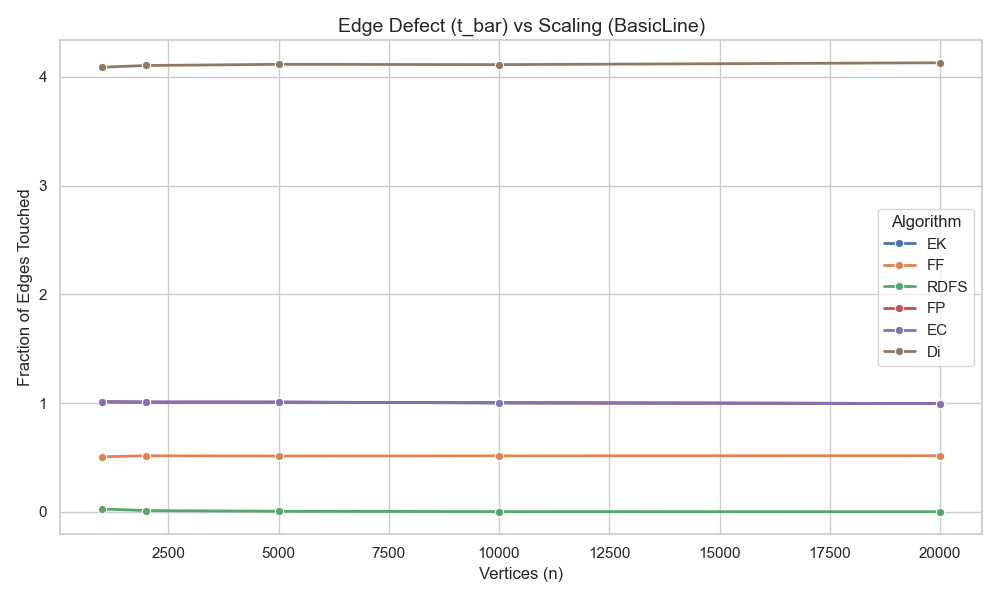
\includegraphics[width=0.75\textwidth]{Images/t_bar_scaling_BasicLine.png}
    \caption{Defeito de Arcos ($\overline{t}$) vs Escala (BasicLine): Mostra que a eficiência de busca por fase permanece estável conforme o número de vértices aumenta. }
\end{figure}




%==================================================
% TABELAS DE RESULTADOS NUMÉRICOS
%==================================================
\subsection{Tabelas de Resultados Numéricos}

As tabelas a seguir complementam os gráficos com os valores brutos coletados para cada
algoritmo, instância e família de grafos. As colunas reportam: número de vértices ($n$),
número de arcos ($m$), fluxo máximo ($C$), fases executadas ($F$), limite teórico
($\overline{F}$), razão de fases ($r = F/\overline{F}$), defeito de vértices
($\overline{s}$), defeito de arcos ($\overline{t}$) e tempo em milissegundos.

% --------------------------------------------------
\subsubsection{DoubleExpLine -- Experimento A (Densidade, $n$ fixo)}
% --------------------------------------------------

\begin{table}[H]
\centering
\caption{DoubleExpLine -- Impacto de Densidade ($n = 5002$, grau $\in \{2,5,10,20,40\}$).}
\resizebox{\textwidth}{!}{%
\begin{tabular}{llrrrrrrrrr}
\toprule
\textbf{Algo} & \textbf{Grau} & \textbf{$m$} & \textbf{$C$} & \textbf{$F$} & \textbf{$\overline{F}$} & \textbf{$r$} & \textbf{$\overline{s}$} & \textbf{$\overline{t}$} & \textbf{ms} \\
\midrule
EK   & 2  & 10040  & 23\,028\,141  & 1204  & 25\,110\,040  & 0.0000 & 0.4500 & 0.9326 & 422.7  \\
FF   & 2  & 10040  & 23\,028\,141  & 2462  & 23\,028\,141  & 0.0001 & 0.2000 & 0.4188 & 880.3  \\
RDFS & 2  & 10040  & 23\,028\,141  & 1490  & 23\,028\,141  & 0.0001 & 0.0213 & 0.0392 & 381.4  \\
FP   & 2  & 10040  & 23\,028\,141  & 1179  & 245\,547       & 0.0048 & 0.1937 & 0.5408 & 411.2  \\
EC   & 2  & 10040  & 23\,028\,141  & 1183  & 245\,547       & 0.0048 & 0.4447 & 0.9228 & 414.9  \\
Di   & 2  & 10040  & 23\,028\,141  &   14  & 5\,002         & 0.0028 & 0.0068 & 2.8606 &  16.0  \\
\midrule
EK   & 5  & 10080  & 52\,796\,313  & 1207  & 25\,210\,080  & 0.0000 & 0.4553 & 0.9311 & 414.5  \\
FF   & 5  & 10080  & 52\,796\,313  & 3238  & 52\,796\,313  & 0.0001 & 0.2302 & 0.4688 & 1282.2 \\
RDFS & 5  & 10080  & 52\,796\,313  & 1581  & 52\,796\,313  & 0.0000 & 0.0157 & 0.0285 & 350.7  \\
FP   & 5  & 10080  & 52\,796\,313  & 1103  & 258\,592       & 0.0043 & 0.2027 & 0.5410 & 413.6  \\
EC   & 5  & 10080  & 52\,796\,313  & 1129  & 258\,592       & 0.0044 & 0.4436 & 0.9080 & 390.3  \\
Di   & 5  & 10080  & 52\,796\,313  &   23  & 5\,002         & 0.0046 & 0.0104 & 2.7947 &  24.8  \\
\midrule
EK   & 10 & 10019  & 100\,463\,419 & 1191  & 25\,057\,519  & 0.0000 & 0.4481 & 0.9200 & 396.6  \\
FF   & 10 & 10019  & 100\,463\,419 & 2775  & 100\,463\,419 & 0.0000 & 0.2128 & 0.4334 & 1000.7 \\
RDFS & 10 & 10019  & 100\,463\,419 & 1566  & 100\,463\,419 & 0.0000 & 0.0096 & 0.0172 & 311.5  \\
FP   & 10 & 10019  & 100\,463\,419 & 1092  & 266\,326       & 0.0041 & 0.2039 & 0.5474 & 459.2  \\
EC   & 10 & 10019  & 100\,463\,419 & 1110  & 266\,326       & 0.0042 & 0.4318 & 0.8881 & 370.9  \\
Di   & 10 & 10019  & 100\,463\,419 &   14  & 5\,002         & 0.0028 & 0.0065 & 2.8104 &  15.3  \\
\midrule
EK   & 20 & 9974   & 184\,772\,843 & 1259  & 24\,944\,974  & 0.0001 & 0.4609 & 0.9349 & 430.3  \\
FF   & 20 & 9974   & 184\,772\,843 & 3510  & 184\,772\,843 & 0.0000 & 0.2228 & 0.4462 & 1272.7 \\
RDFS & 20 & 9974   & 184\,772\,843 & 1853  & 184\,772\,843 & 0.0000 & 0.0080 & 0.0143 & 360.7  \\
FP   & 20 & 9974   & 184\,772\,843 & 1117  & 273\,898       & 0.0041 & 0.2540 & 0.6158 & 693.6  \\
EC   & 20 & 9974   & 184\,772\,843 & 1145  & 273\,898       & 0.0042 & 0.4335 & 0.8823 & 381.6  \\
Di   & 20 & 9974   & 184\,772\,843 &   11  & 5\,002         & 0.0022 & 0.0051 & 2.8406 &  12.0  \\
\midrule
EK   & 40 & 10131  & 298\,734\,032 & 1288  & 25\,337\,631  & 0.0001 & 0.4722 & 0.9515 & 445.7  \\
FF   & 40 & 10131  & 298\,734\,032 & 2458  & 298\,734\,032 & 0.0000 & 0.2261 & 0.4491 & 920.7  \\
RDFS & 40 & 10131  & 298\,734\,032 & 1789  & 298\,734\,032 & 0.0000 & 0.0073 & 0.0130 & 344.0  \\
FP   & 40 & 10131  & 298\,734\,032 & 1133  & 285\,231       & 0.0040 & 0.3373 & 0.7417 & 1032.2 \\
EC   & 40 & 10131  & 298\,734\,032 & 1172  & 285\,231       & 0.0041 & 0.4391 & 0.8880 & 387.0  \\
Di   & 40 & 10131  & 298\,734\,032 &    7  & 5\,002         & 0.0014 & 0.0034 & 2.8601 &   7.7  \\
\bottomrule
\end{tabular}}
\end{table}

% --------------------------------------------------
\subsubsection{DoubleExpLine -- Experimento B (Escala, densidade fixa)}
% --------------------------------------------------

\begin{table}[H]
\centering
\caption{DoubleExpLine -- Impacto de Escala (grau fixo $= 10$, $n \in \{1002, 2002, 5002, 10002, 20002\}$).}
\resizebox{\textwidth}{!}{%
\begin{tabular}{llrrrrrrrrr}
\toprule
\textbf{Algo} & \textbf{$n$} & \textbf{$m$} & \textbf{$C$} & \textbf{$F$} & \textbf{$\overline{F}$} & \textbf{$r$} & \textbf{$\overline{s}$} & \textbf{$\overline{t}$} & \textbf{ms} \\
\midrule
EK   & 1002  & 1990   & 18\,709\,209  &   211 & 996\,990      & 0.0002 & 0.4485 & 0.9234 &    12.0 \\
FF   & 1002  & 1990   & 18\,709\,209  &   426 & 18\,709\,209  & 0.0000 & 0.2491 & 0.4996 &    34.1 \\
RDFS & 1002  & 1990   & 18\,709\,209  &   281 & 18\,709\,209  & 0.0000 & 0.0293 & 0.0522 &    15.9 \\
FP   & 1002  & 1990   & 18\,709\,209  &   201 & 48\,073        & 0.0042 & 0.2049 & 0.5477 &    15.3 \\
EC   & 1002  & 1990   & 18\,709\,209  &   204 & 48\,073        & 0.0042 & 0.4326 & 0.8939 &    11.9 \\
Di   & 1002  & 1990   & 18\,709\,209  &     8 & 1\,002         & 0.0080 & 0.0214 & 2.8333 &     1.7 \\
\midrule
EK   & 2002  & 4038   & 41\,334\,988  &   493 & 4\,042\,038   & 0.0001 & 0.4512 & 0.9263 &    60.5 \\
FF   & 2002  & 4038   & 41\,334\,988  &  1059 & 41\,334\,988  & 0.0000 & 0.2128 & 0.4284 &   150.4 \\
RDFS & 2002  & 4038   & 41\,334\,988  &   652 & 41\,334\,988  & 0.0000 & 0.0192 & 0.0338 &    62.5 \\
FP   & 2002  & 4038   & 41\,334\,988  &   453 & 102\,165       & 0.0044 & 0.2237 & 0.5788 &    82.6 \\
EC   & 2002  & 4038   & 41\,334\,988  &   455 & 102\,165       & 0.0045 & 0.4342 & 0.8932 &    56.9 \\
Di   & 2002  & 4038   & 41\,334\,988  &    11 & 2\,002         & 0.0055 & 0.0130 & 2.8449 &     4.9 \\
\midrule
EK   & 5002  & 10019  & 100\,463\,419 &  1191 & 25\,057\,519  & 0.0000 & 0.4481 & 0.9200 &   400.8 \\
FF   & 5002  & 10019  & 100\,463\,419 &  2775 & 100\,463\,419 & 0.0000 & 0.2128 & 0.4334 &   984.2 \\
RDFS & 5002  & 10019  & 100\,463\,419 &  1537 & 100\,463\,419 & 0.0000 & 0.0100 & 0.0180 &   312.1 \\
FP   & 5002  & 10019  & 100\,463\,419 &  1092 & 266\,326       & 0.0041 & 0.2039 & 0.5474 &   457.7 \\
EC   & 5002  & 10019  & 100\,463\,419 &  1110 & 266\,326       & 0.0042 & 0.4318 & 0.8881 &   370.6 \\
Di   & 5002  & 10019  & 100\,463\,419 &    14 & 5\,002         & 0.0028 & 0.0065 & 2.8104 &    15.3 \\
\midrule
EK   & 10002 & 19957  & 198\,789\,778 &  2390 & 99\,804\,957  & 0.0000 & 0.4544 & 0.9321 &  1725.6 \\
FF   & 10002 & 19957  & 198\,789\,778 &  4914 & 198\,789\,778 & 0.0000 & 0.2157 & 0.4412 &  3635.5 \\
RDFS & 10002 & 19957  & 198\,789\,778 &  3315 & 198\,789\,778 & 0.0000 & 0.0061 & 0.0112 &  1268.7 \\
FP   & 10002 & 19957  & 198\,789\,778 &  2153 & 550\,148       & 0.0039 & 0.2065 & 0.5496 &  1936.2 \\
EC   & 10002 & 19957  & 198\,789\,778 &  2197 & 550\,148       & 0.0040 & 0.4361 & 0.8966 &  1588.4 \\
Di   & 10002 & 19957  & 198\,789\,778 &    17 & 10\,002        & 0.0017 & 0.0039 & 2.8030 &    37.5 \\
\midrule
EK   & 20002 & 40158  & 392\,986\,397 &  4711 & 401\,620\,158 & 0.0000 & 0.4543 & 0.9294 &  7287.6 \\
FF   & 20002 & 40158  & 392\,986\,397 & 13337 & 392\,986\,397 & 0.0000 & 0.2289 & 0.4649 & 21329.5 \\
RDFS & 20002 & 40158  & 392\,986\,397 &  6666 & 392\,986\,397 & 0.0000 & 0.0042 & 0.0079 &  4895.3 \\
FP   & 20002 & 40158  & 392\,986\,397 &  4294 & 1\,146\,507   & 0.0037 & 0.2179 & 0.5676 &  8575.0 \\
EC   & 20002 & 40158  & 392\,986\,397 &  4384 & 1\,146\,507   & 0.0038 & 0.4366 & 0.8948 &  6645.4 \\
Di   & 20002 & 40158  & 392\,986\,397 &    18 & 20\,002        & 0.0009 & 0.0021 & 2.7839 &    81.8 \\
\bottomrule
\end{tabular}}
\end{table}

% --------------------------------------------------
\subsubsection{BasicLine -- Experimento A (Densidade, $n$ fixo)}
% --------------------------------------------------

\begin{table}[H]
\centering
\caption{BasicLine -- Impacto de Densidade ($n = 5002$, grau $\in \{2,5,10,20,40\}$).}
\resizebox{\textwidth}{!}{%
\begin{tabular}{llrrrrrrrrr}
\toprule
\textbf{Algo} & \textbf{Grau} & \textbf{$m$} & \textbf{$C$} & \textbf{$F$} & \textbf{$\overline{F}$} & \textbf{$r$} & \textbf{$\overline{s}$} & \textbf{$\overline{t}$} & \textbf{ms} \\
\midrule
EK   & 2  & 10067 & 12\,313\,496 & 2521 & 25\,177\,567 & 0.0001 & 0.5039 & 1.0101 &   838.0 \\
FF   & 2  & 10067 & 12\,313\,496 & 3631 & 12\,313\,496 & 0.0003 & 0.2621 & 0.5254 &  1516.7 \\
RDFS & 2  & 10067 & 12\,313\,496 & 3731 & 12\,313\,496 & 0.0003 & 0.0036 & 0.0059 &   655.8 \\
FP   & 2  & 10067 & 12\,313\,496 & 2495 & 237\,115      & 0.0105 & 0.5007 & 1.0054 &  4462.4 \\
EC   & 2  & 10067 & 12\,313\,496 & 2504 & 237\,115      & 0.0106 & 0.5004 & 1.0032 &   839.3 \\
Di   & 2  & 10067 & 12\,313\,496 &    2 & 5\,002        & 0.0004 & 0.0010 & 3.5349 &     3.0 \\
\midrule
EK   & 5  & 10014 & 12\,155\,227 & 2422 & 25\,045\,014 & 0.0001 & 0.5002 & 1.0094 &   825.4 \\
FF   & 5  & 10014 & 12\,155\,227 & 3460 & 12\,155\,227 & 0.0003 & 0.2560 & 0.5185 &  1453.8 \\
RDFS & 5  & 10014 & 12\,155\,227 & 3723 & 12\,155\,227 & 0.0003 & 0.0038 & 0.0063 &   659.9 \\
FP   & 5  & 10014 & 12\,155\,227 & 2422 & 235\,680      & 0.0103 & 0.5005 & 1.0095 &  4270.9 \\
EC   & 5  & 10014 & 12\,155\,227 & 2422 & 235\,680      & 0.0103 & 0.5002 & 1.0094 &   827.7 \\
Di   & 5  & 10014 & 12\,155\,227 &    1 & 5\,002        & 0.0002 & 0.0008 & 4.0904 &     2.0 \\
\midrule
EK   & 10 & 10003 & 12\,519\,952 & 2485 & 25\,017\,503 & 0.0001 & 0.5002 & 1.0090 &   862.9 \\
FF   & 10 & 10003 & 12\,519\,952 & 3502 & 12\,519\,952 & 0.0003 & 0.2542 & 0.5138 &  1412.3 \\
RDFS & 10 & 10003 & 12\,519\,952 & 3785 & 12\,519\,952 & 0.0003 & 0.0037 & 0.0061 &   666.9 \\
FP   & 10 & 10003 & 12\,519\,952 & 2485 & 235\,848      & 0.0105 & 0.5005 & 1.0091 &  4353.4 \\
EC   & 10 & 10003 & 12\,519\,952 & 2485 & 235\,848      & 0.0105 & 0.5002 & 1.0090 &   864.4 \\
Di   & 10 & 10003 & 12\,519\,952 &    1 & 5\,002        & 0.0002 & 0.0008 & 4.1145 &     2.0 \\
\midrule
EK   & 20 & 10109 & 12\,529\,519 & 2529 & 25\,282\,609 & 0.0001 & 0.5002 & 1.0040 &   869.6 \\
FF   & 20 & 10109 & 12\,529\,519 & 3540 & 12\,529\,519 & 0.0003 & 0.2554 & 0.5112 &  1490.7 \\
RDFS & 20 & 10109 & 12\,529\,519 & 3866 & 12\,529\,519 & 0.0003 & 0.0035 & 0.0058 &   690.0 \\
FP   & 20 & 10109 & 12\,529\,519 & 2529 & 238\,358      & 0.0106 & 0.5005 & 1.0041 &  4448.2 \\
EC   & 20 & 10109 & 12\,529\,519 & 2529 & 238\,358      & 0.0106 & 0.5002 & 1.0040 &   882.1 \\
Di   & 20 & 10109 & 12\,529\,519 &    1 & 5\,002        & 0.0002 & 0.0008 & 4.1279 &     1.9 \\
\midrule
EK   & 40 & 10007 & 12\,083\,885 & 2436 & 25\,027\,507 & 0.0001 & 0.5002 & 1.0019 &   834.4 \\
FF   & 40 & 10007 & 12\,083\,885 & 3510 & 12\,083\,885 & 0.0003 & 0.2620 & 0.5220 &  1429.8 \\
RDFS & 40 & 10007 & 12\,083\,885 & 3689 & 12\,083\,885 & 0.0003 & 0.0034 & 0.0056 &   656.7 \\
FP   & 40 & 10007 & 12\,083\,885 & 2436 & 235\,431      & 0.0103 & 0.5005 & 1.0021 &  4259.7 \\
EC   & 40 & 10007 & 12\,083\,885 & 2436 & 235\,431      & 0.0103 & 0.5002 & 1.0019 &   837.6 \\
Di   & 40 & 10007 & 12\,083\,885 &    1 & 5\,002        & 0.0002 & 0.0008 & 4.0997 &     2.0 \\
\bottomrule
\end{tabular}}
\end{table}

% --------------------------------------------------
\subsubsection{BasicLine -- Experimento B (Escala, densidade fixa)}
% --------------------------------------------------

\begin{table}[H]
\centering
\caption{BasicLine -- Impacto de Escala (grau fixo $= 10$, $n \in \{1002, 2002, 5002, 10002, 20002\}$).}
\resizebox{\textwidth}{!}{%
\begin{tabular}{llrrrrrrrrr}
\toprule
\textbf{Algo} & \textbf{$n$} & \textbf{$m$} & \textbf{$C$} & \textbf{$F$} & \textbf{$\overline{F}$} & \textbf{$r$} & \textbf{$\overline{s}$} & \textbf{$\overline{t}$} & \textbf{ms} \\
\midrule
EK   & 1002  & 2020  & 2\,410\,324  &    474 & 1\,012\,020   & 0.0005 & 0.5010 & 1.0119 &    27.7 \\
FF   & 1002  & 2020  & 2\,410\,324  &    694 & 2\,410\,324   & 0.0003 & 0.2512 & 0.5071 &    56.3 \\
RDFS & 1002  & 2020  & 2\,410\,324  &    747 & 2\,410\,324   & 0.0003 & 0.0161 & 0.0265 &    34.2 \\
FP   & 1002  & 2020  & 2\,410\,324  &    474 & 42\,826        & 0.0111 & 0.5023 & 1.0124 &   138.8 \\
EC   & 1002  & 2020  & 2\,410\,324  &    474 & 42\,826        & 0.0111 & 0.5010 & 1.0119 &    27.8 \\
Di   & 1002  & 2020  & 2\,410\,324  &      1 & 1\,002         & 0.0010 & 0.0042 & 4.0881 &     0.4 \\
\midrule
EK   & 2002  & 3989  & 4\,856\,178  &    988 & 3\,992\,989   & 0.0002 & 0.5005 & 1.0093 &   124.1 \\
FF   & 2002  & 3989  & 4\,856\,178  &   1365 & 4\,856\,178   & 0.0003 & 0.2556 & 0.5160 &   226.5 \\
RDFS & 2002  & 3989  & 4\,856\,178  &   1467 & 4\,856\,178   & 0.0003 & 0.0077 & 0.0126 &   113.2 \\
FP   & 2002  & 3989  & 4\,856\,178  &    988 & 88\,601        & 0.0112 & 0.5011 & 1.0096 &   620.1 \\
EC   & 2002  & 3989  & 4\,856\,178  &    988 & 88\,601        & 0.0112 & 0.5005 & 1.0093 &   124.4 \\
Di   & 2002  & 3989  & 4\,856\,178  &      1 & 2\,002         & 0.0005 & 0.0021 & 4.1038 &     0.8 \\
\midrule
EK   & 5002  & 10003 & 12\,519\,952 &   2485 & 25\,017\,503  & 0.0001 & 0.5002 & 1.0090 &   855.6 \\
FF   & 5002  & 10003 & 12\,519\,952 &   3502 & 12\,519\,952  & 0.0003 & 0.2542 & 0.5138 &  1412.5 \\
RDFS & 5002  & 10003 & 12\,519\,952 &   3786 & 12\,519\,952  & 0.0003 & 0.0037 & 0.0062 &   658.9 \\
FP   & 5002  & 10003 & 12\,519\,952 &   2485 & 235\,848       & 0.0105 & 0.5005 & 1.0091 &  4350.1 \\
EC   & 5002  & 10003 & 12\,519\,952 &   2485 & 235\,848       & 0.0105 & 0.5002 & 1.0090 &   859.3 \\
Di   & 5002  & 10003 & 12\,519\,952 &      1 & 5\,002         & 0.0002 & 0.0008 & 4.1145 &     2.1 \\
\midrule
EK   & 10002 & 19904 & 24\,355\,876 &   4903 & 99\,539\,904  & 0.0000 & 0.5001 & 1.0030 &  3557.9 \\
FF   & 10002 & 19904 & 24\,355\,876 &   6973 & 24\,355\,876  & 0.0003 & 0.2576 & 0.5156 &  5649.4 \\
RDFS & 10002 & 19904 & 24\,355\,876 &   7273 & 24\,355\,876  & 0.0003 & 0.0018 & 0.0031 &  2512.5 \\
FP   & 10002 & 19904 & 24\,355\,876 &   4903 & 488\,400       & 0.0100 & 0.5002 & 1.0031 & 18359.6 \\
EC   & 10002 & 19904 & 24\,355\,876 &   4903 & 488\,400       & 0.0100 & 0.5001 & 1.0030 &  3583.7 \\
Di   & 10002 & 19904 & 24\,355\,876 &      1 & 10\,002        & 0.0001 & 0.0004 & 4.1118 &     4.0 \\
\midrule
EK   & 20002 & 40105 & 50\,204\,624 &  10124 & 401\,090\,105 & 0.0000 & 0.5000 & 0.9967 & 15274.1 \\
FF   & 20002 & 40105 & 50\,204\,624 &  14285 & 50\,204\,624  & 0.0003 & 0.2596 & 0.5165 & 23560.8 \\
RDFS & 20002 & 40105 & 50\,204\,624 &  14916 & 50\,204\,624  & 0.0003 & 0.0011 & 0.0019 & 10353.8 \\
FP   & 20002 & 40105 & 50\,204\,624 &  10124 & 1\,025\,939   & 0.0099 & 0.5001 & 0.9968 & 81648.3 \\
EC   & 20002 & 40105 & 50\,204\,624 &  10124 & 1\,025\,939   & 0.0099 & 0.5000 & 0.9967 & 15448.2 \\
Di   & 20002 & 40105 & 50\,204\,624 &      1 & 20\,002        & 0.0000 & 0.0002 & 4.1287 &     8.3 \\
\bottomrule
\end{tabular}}
\end{table}



%==================================================
% ANÁLISE QUANTITATIVA DA DEFICIÊNCIA
%==================================================
\section{Análise Quantitativa da Deficiência}

Esta seção analisa sistematicamente as três métricas de defeito — $r$, $\overline{s}$ e
$\overline{t}$ — para cada algoritmo, confrontando os valores experimentais com os limites
teóricos pessimistas.

% --------------------------------------------------
\subsection{Inadequação de Fases ($r = F / \overline{F}$)}
% --------------------------------------------------

A métrica $r$ quantifica o quanto o número real de fases fica abaixo do limite teórico.
Valores próximos de zero indicam que o limite pessimista é extremamente frouxo.

\textbf{Edmonds-Karp (EK).} O limite teórico $\overline{F} = nm/2$ é o mais conservador
do conjunto. Em todas as instâncias, $r < 0{,}0001$, chegando a $r = 0{,}0000$ para
redes grandes. No experimento de escala (DoubleExpLine), com $n = 20002$ e $m = 40158$,
o limite é $\overline{F} \approx 401{,}6 \times 10^6$, enquanto o algoritmo executa
apenas $4711$ fases — uma inadequação de cinco ordens de magnitude.

\textbf{Ford-Fulkerson DFS e RDFS.} Esses algoritmos usam $\overline{F} = C$ (fluxo
máximo). Apesar de $C$ ser muito menor do que $nm/2$, ainda assim $r$ permanece
inferior a $0{,}0003$ em todas as instâncias. O fluxo máximo é da ordem de $10^7$--$10^8$,
enquanto o número real de fases é de poucos milhares. Notavelmente, RDFS executa menos
fases que FF em todas as instâncias de DoubleExpLine (e.g., 1490 vs 2462 para grau 2),
evidenciando que o embaralhamento aleatoriza efetivamente os caminhos, reduzindo o
número de iterações.

\textbf{Fattest Path (FP) e Escalonamento de Capacidade (EC).} Compartilham o limite
$\overline{F} = m \log_2 C$. Os valores de $r$ são os maiores do conjunto, em torno de
$0{,}004$--$0{,}011$, o que indica que o limite $m \log_2 C$ é mais preciso
relativamente às demais estratégias, mas ainda superestima as fases reais por dois
a três ordens de magnitude. Na BasicLine com $n = 20002$, $\overline{F} \approx 10^6$,
enquanto ambos executam $10124$ fases ($r \approx 0{,}010$).

\textbf{Dinitz (Di).} Usa $\overline{F} = n$. É o algoritmo com a melhor relação entre
fases reais e limite teórico. Na BasicLine, o número de fases é consistentemente
$F = 1$ (uma única fase BFS + fluxo bloqueante já satura a rede), resultando em
$r \leq 0{,}001$ independente de $n$. Na DoubleExpLine, onde a estrutura é mais
complexa, $F$ chega a $23$ (para grau 5), mas o limite $\overline{F} = n = 5002$
ainda implica $r = 0{,}0046$. A Tabela~5 resume a evolução de $r$ com $n$ para Dinitz:

\begin{table}[H]
\centering
\caption{Dinitz: $F$ real vs.\ $\overline{F} = n$ por família e escala.}
\begin{tabular}{lrrrr}
\toprule
\textbf{Família} & \textbf{$n$} & \textbf{$F$} & \textbf{$\overline{F}$} & \textbf{$r$} \\
\midrule
DoubleExpLine & 1002  & 8  & 1002  & 0.0080 \\
DoubleExpLine & 2002  & 11 & 2002  & 0.0055 \\
DoubleExpLine & 5002  & 14 & 5002  & 0.0028 \\
DoubleExpLine & 10002 & 17 & 10002 & 0.0017 \\
DoubleExpLine & 20002 & 18 & 20002 & 0.0009 \\
\midrule
BasicLine     & 1002  & 1  & 1002  & 0.0010 \\
BasicLine     & 2002  & 1  & 2002  & 0.0005 \\
BasicLine     & 5002  & 1  & 5002  & 0.0002 \\
BasicLine     & 10002 & 1  & 10002 & 0.0001 \\
BasicLine     & 20002 & 1  & 20002 & 0.0000 \\
\bottomrule
\end{tabular}
\end{table}

Na DoubleExpLine, $F$ cresce de forma logarítmica com $n$ (de 8 a 18 quando $n$
quadruplica de 1002 a 20002), enquanto $\overline{F} = n$ cresce linearmente —
confirmando empiricamente que Dinitz opera muito abaixo do seu pior caso.

% --------------------------------------------------
\subsection{Defeito de Vértices ($\overline{s}$)}
% --------------------------------------------------

O defeito $\overline{s}$ mede a fração média de vértices da rede que são tocados por
fase (ou por iteração interna, no caso de Dinitz). Cada algoritmo revela um padrão
distinto e estável entre instâncias.

\textbf{EK} apresenta $\overline{s} \approx 0{,}45$--$0{,}50$ em todas as instâncias
e famílias. Isso reflete a natureza da BFS: em cada fase ela percorre praticamente
metade da rede em largura antes de alcançar o sorvedouro.

\textbf{FF} mantém $\overline{s} \approx 0{,}21$--$0{,}26$: a DFS encontra caminhos
mais curtos em média, tocando cerca de $1/4$ dos vértices por fase.

\textbf{RDFS} apresenta $\overline{s}$ extremamente baixo, decrescendo de
$\approx 0{,}016$--$0{,}029$ em redes pequenas a $\approx 0{,}001$--$0{,}004$ em
$n = 20002$. O embaralhamento aleatório faz com que a DFS encontre caminhos muito
curtos em média, tocando uma fração ínfima dos vértices.

\textbf{FP} e \textbf{EC} têm comportamentos distintos entre si: EC converge para
$\overline{s} \approx 0{,}43$--$0{,}50$ (similar a EK, pois também usa BFS na busca
por caminhos), enquanto FP apresenta maior variabilidade ($0{,}19$--$0{,}50$),
refletindo a dependência da estrutura de capacidades na escolha do caminho mais gordo.

\textbf{Dinitz} tem $\overline{s}$ muito baixo ($< 0{,}02$ na DoubleExpLine,
$< 0{,}005$ na BasicLine), pois o divisor é o número total de iterações internas — que
é muito maior que o número de fases — e cada iteração individual da DFS de fluxo
bloqueante percorre um subconjunto pequeno de vértices do grafo de níveis.

% --------------------------------------------------
\subsection{Defeito de Arcos ($\overline{t}$)}
% --------------------------------------------------

O defeito $\overline{t}$ mede a fração de arcos avaliados por fase em relação ao total
$m$. Valores acima de $1{,}0$ indicam que, em média, cada arco é avaliado mais de uma
vez por fase — o que ocorre quando o algoritmo realiza múltiplas travessias por fase
(como Dinitz com seu fluxo bloqueante).

\textbf{EK} apresenta $\overline{t} \approx 0{,}92$--$1{,}01$: em cada fase BFS quase
todos os arcos são examinados, o que é esperado dado que a BFS visita camadas
sucessivas de forma exaustiva.

\textbf{FF} mantém $\overline{t} \approx 0{,}41$--$0{,}52$: a DFS encontra um caminho
e para, avaliando cerca de metade dos arcos por fase.

\textbf{RDFS} apresenta $\overline{t}$ muito baixo e decrescente com $n$: de
$\approx 0{,}027$ em redes menores a $\approx 0{,}002$ com $n = 20002$. O embaralhamento
produz caminhos curtos que percorrem uma fração mínima dos arcos.

\textbf{FP} opera com $\overline{t} \approx 0{,}54$--$0{,}74$: o algoritmo de Dijkstra
modificado avalia mais arcos que a DFS pura, pois mantém uma fila de prioridade e
relaxa arestas múltiplas vezes por fase.

\textbf{EC} apresenta $\overline{t} \approx 0{,}88$--$0{,}95$ na maioria das instâncias,
próximo de EK, pois também usa BFS porém restrita a arcos com capacidade residual
$\geq \Delta$, o que não reduz significativamente o número de arcos examinados.

\textbf{Dinitz} é o único algoritmo com $\overline{t}$ consistentemente \emph{acima}
de $1{,}0$: os valores ficam entre $2{,}78$ e $4{,}13$. Isso ocorre porque cada fase
de Dinitz realiza múltiplas iterações de DFS sobre o grafo de níveis, resultando em
múltiplas travessias do grafo por fase. A BasicLine apresenta valores maiores
($\approx 4{,}1$) que a DoubleExpLine ($\approx 2{,}8$), pois na BasicLine uma única
fase já satura completamente a rede, exigindo um número maior de iterações internas.

% --------------------------------------------------
\subsection{Síntese Comparativa}
% --------------------------------------------------

\begin{table}[H]
\centering
\caption{Médias das métricas de defeito por algoritmo (todas as instâncias).}
\begin{tabular}{lrrrr}
\toprule
\textbf{Algoritmo} & \textbf{$\overline{r}$ (médio)} & \textbf{$\overline{s}$ (médio)} & \textbf{$\overline{t}$ (médio)} & \textbf{Interpretação} \\
\midrule
EK   & $9 \times 10^{-5}$ & 0.4775 & 0.9683 & BFS exaustiva, poucas fases reais \\
FF   & $2 \times 10^{-4}$ & 0.2390 & 0.4822 & DFS profunda, fases moderadas \\
RDFS & $1{,}5 \times 10^{-4}$ & 0.0090 & 0.0158 & Caminhos curtos, mínimo de arcos \\
FP   & $7{,}3 \times 10^{-3}$ & 0.3628 & 0.7920 & Maior $r$ relativo, heap custoso \\
EC   & $7{,}4 \times 10^{-3}$ & 0.4683 & 0.9507 & Comportamento próximo a EK \\
Di   & $1{,}8 \times 10^{-3}$ & 0.0046 & 3.4378 & Pouquíssimas fases, múltiplos arcos/fase \\
\bottomrule
\end{tabular}
\end{table}

Os dados revelam uma tensão fundamental entre as métricas: algoritmos que executam
poucas fases (como EK e Dinitz) tendem a tocar mais arcos por fase ($\overline{t}$
alto), enquanto algoritmos com muitas fases (como RDFS) tocam uma fração mínima dos
arcos a cada iteração ($\overline{t}$ baixo). O ponto ótimo de eficiência prática
— medido pelo tempo total — é alcançado pelo Dinitz, que combina número mínimo de
fases com custo por fase bem controlado, apesar de $\overline{t} > 1$. O Fattest
Path, embora use um limite $\overline{F}$ mais preciso que EK e os métodos DFS, paga
um custo elevado por fase devido à manutenção do Max-Heap, o que explica seu desempenho
temporal inferior ao EC apesar de executarem o mesmo número de fases.

%==================================================
% CONLUSÃO
%==================================================
\section{Conclusão}
Os experimentos confirmam que os limites teóricos pessimistas são inadequados para prever o desempenho em instâncias práticas. O algoritmo de Dinitz destacou-se pela alta eficiência em todas as topologias, enquanto o Fattest Path, apesar de sua elegância matemática, sofre com a sobrecarga residual de manter estruturas de dados complexas como o Max-Heap.

\end{document}